\documentclass[11pt, oneside]{article} 
\usepackage{geometry}
\geometry{letterpaper} 
\usepackage{graphicx}
	
\usepackage{amssymb}
\usepackage{amsmath}
\usepackage{parskip}
\usepackage{color}
\usepackage{hyperref}

\graphicspath{{/Users/telliott/Github/calculus_book/png/}}
% \begin{center} 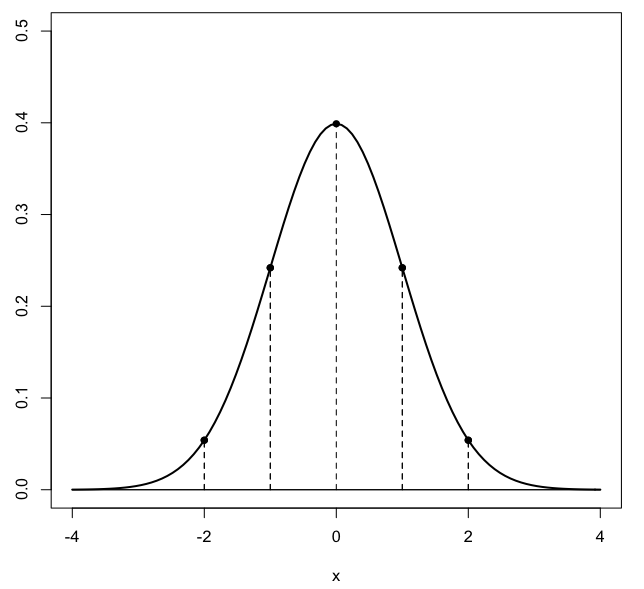
\includegraphics [scale=0.4] {gauss3.png} \end{center}

\title{Triangle inequality}
\date{}

\begin{document}
\maketitle
\Large

\section*{Introduction}

Here we prove the theorem known as the \textbf{triangle inequality}, which is used in proving numerous other theorems in analysis.  It involves the concept of absolute value.

\subsection*{Absolute value}

The absolute value function is typeset as $|x|$ and defined as follows:
\[
f(x) = |x| = 
\begin{cases}
\ \ 0, \ \ \ x = 0 \\
\ \ x, \ \ \ x > 0 \\
-x, \ \ \ x < 0
\end{cases}
\]

The definition can be simplified by combining the first two cases into one statement:  $|x| = x$ for $x \ge 0$.  But in what follows we will usually consider the three cases separately.

\subsection*{theorem}
We will prove that 
\[ |x + y| \le |x| + |y| \] 

This inequality holds regardless of the signs of $x$ and $y$.

\subsection*{Aside on geometry}
The triangle inequality is named after the version from geometry.  

When considering the lengths of the sides of a triangle (or the distances between three points in the plane), the lengths of any two sides added together are greater than the length of the third side.  Equality is found for the limiting case when the triangle collapses.

\begin{center} 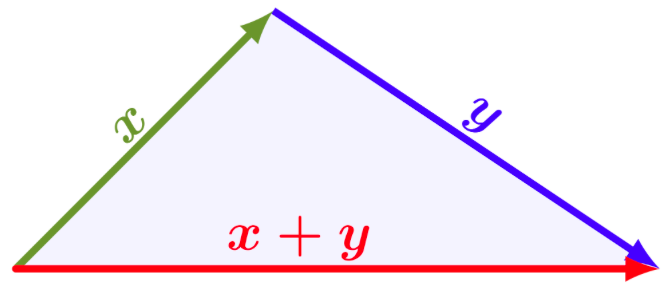
\includegraphics [scale=0.3] {triangle_inequality.png} \end{center}

Euclid teaches us that the shortest distance between any two points is a straight line (in this figure from the web, $\mathbf{x + y}$ refers to the \emph{vector sum} of $\mathbf{x}$ and $\mathbf{y}$).

For the real number line, consider any set of three points.  The largest distance is equal to the other two added together
\begin{center} 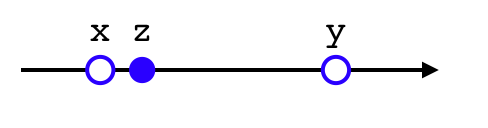
\includegraphics [scale=0.4] {3points.png} \end{center}
\[ d(x,y) = d(x,z) + d(z,y) \]
Any other single distance is less than the sum of the remaining two.

For points in $R^1$ the absolute value gives the distance between them.  For vectors in $R^2$ the absolute value gives the length (which is also the distance between vertices).

One way to prove the theorem
\[ |x + y| \le |x| + |y| \] 

is to go through cases.  It turns out that if $x$ and $y$ are both positive or both negative, the above relationship is an equality, equivalent to what we said above about the largest distance is equal to the other two added together.

It is only when the terms have opposite signs that the result is $<$.  

For a formal approach (especially helpful for the case of different signs), we follow Apostol.  We consider a preliminary theorem first, which is another result frequently used in analysis.

\section*{Interval with midpoint}

Consider an open interval whose endpoints are equidistant from a central point $p$, where the distance to the boundary is $a$ (as a \emph{distance}, certainly $a > 0$), and  $x$ is contained somewhere in the open interval $(p-a,p+a)$

\begin{center} 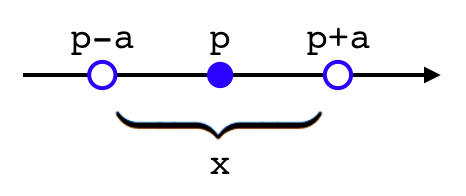
\includegraphics [scale=0.4] {neighborhood2.png} \end{center}

We can translate this picture to algebra as
\[ p - a < x < p + a \]
Adding $-p$ to each term
\[ -a < x - p < a \]

The preliminary theorem states that the above is true if and only if
\[ |x - p| < a  \]
We should read the last statement as saying that the distance between $x$ and $p$ is less than $a$.

Taking the statements above
\[ |x - p| \le a \iff -a \le x - p \le a \]
and rewriting $x -p$ as just $x$ we obtain:  
\[ |x| \le a \iff -a \le x \le a \]
This is the statement we will prove.

\subsubsection*{preliminary preliminary theorem}

There is actually another theorem that comes before the preliminary theorem.
\[ -|x| \le x \le |x| \]

\subsubsection*{proof}

We just do this one by cases.

$\circ$   If $x \ge 0$ then $x = |x|$ and $-|x| < 0$ so $x \ge -|x|$.

$\circ$   If $x < 0$, then $|x|=-x$ and $x = -|x|$ and also $|x| \ge 0$ so $x < |x|$.

\subsection*{preliminary theorem}

\[ |x| \le a \iff -a \le x \le a \]

\subsection*{proof}
Let $a$ be a constant real number $a > 0$ and the starting proposition is
\[ |x| \le a \]
Add the expression $-a - |x|$ to both sides to obtain
\[ -a \le - |x| \]

From the preliminary preliminary theorem we obtain
\[ -|x| \le x \le |x| \]

We combine all three parts:
\[ -a \le -|x| \le x \le |x| \le a \]
which simplifies to
\[ -a \le x \le a \]
This completes the forward proof.

To prove the converse, we are assuming that
\[ x \le a \]
and
\[ - a \le x \]
Now if $x \ge 0$ we have $|x| = x$ so
\[ |x| = x \le a \]
On the other hand for $x < 0$, we start with the first part
\[ -a \le x \]
Add $a - x$ to both sides
\[ -x \le a \]
and since $x < 0$, $|x| = -x$ and we have 
\[ |x| =  -x \le a \]
In both cases we have \[ |x| \le a \]
and this completes the proof.

$\square$

\subsection*{continuity example}

\begin{center} 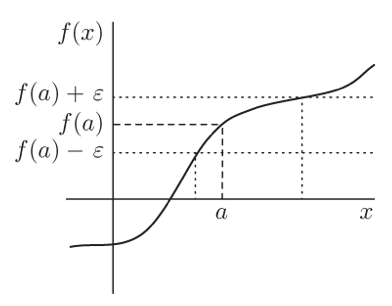
\includegraphics [scale=0.6] {continuity3.png} \end{center}

As motivation for this whole topic, in the definition of \textbf{continuity} of a function $f(x)$ at a point $a$, we play the epsilon-delta game.  Choose an \emph{arbitrary} positive real number $\epsilon > 0$.  

Then we say, $f$ is continuous at $a$ if and only if we can find $\delta$ such that 
\[ |x - a| < \delta \Rightarrow |f(x) - f(a)| < \epsilon \]

If the distance (or difference) between $x$ and $a$ is less than $\delta$, then it follows that the difference $|f(x) - f(a)|$ is less than $\epsilon$.

The last statement is exactly the same as
\[ -\epsilon < f(x) - f(a) < \epsilon \]

The advantage of this formulation is that there are no absolute value signs so we can rearrange the above to give:

\[ f(a) -\epsilon < f(x) < f(a) + \epsilon \]

We will see multiple examples of this in real analysis.

\subsection*{alternative proof (by examining cases)}
The statement
\[ -a < x - p < a \Rightarrow  |x - p| < a  \]
may be proved informally by going exhaustively through the cases, as follows.

(1) If $x = p$ then $x - p = 0 < a$ and $0 > -a$; 

(2) If $x > p$, then $x - p > 0$ and so 
\[ |x - p| = x - p \]
Then
\[ x - p < a \] 
implies 
\[ |x - p| = x - p < a \]
and since the absolute value is positive it is certainly $> -a$.

(3) If $x < p$ then $x - p < 0$ so
\[ |x - p| = -(x-p) = p - x \]
Then the first part of the assumption is
\[ -a < x - p \] 
Add $a + p - x$ to both sides
\[ p - x < a \]
which implies
\[ |x - p| = p - x < a \]
and again the absolute value is positive so it is certainly $> -a$.

This proves the theorem.

$\square$

\section*{Triangle inequality}

Let us change the notation of the previous theorem so we can reuse the variable $x$ in the next part:
\[ | \phi | \le a \iff -a \le \phi \le a \]

Now start by considering
\[ - |x| \le x \le |x| \]
Now add two such inequalities 
\[ - \ [ \ |x| +  |y| \ ] \  \le x + y \le  |x| + |y|  \]

Recall the theorem we just proved with its new notation and focus on the right-hand side
\[  -a \le \phi \le a \]
Equate $a$ with $|x| + |y|$ and $\phi$ with $x + y$.  

Then the expression that we had above by adding two inequalities
\[ - \ [ \ |x| +  |y| \ ] \  \le x + y \le  |x| + |y|  \]
can be seen as equivalent to the right-hand side from the theorem.  
\[  -a \le \phi \le a \]

Therefore, the left-hand side must also be true, namely
\[ |\phi| \le a \]
\[ |x + y| \le  |x| +  |y| \]
This proves the triangle inequality.

$\square$

\subsection*{alternative proof (by examining cases)}

Let $m > n > 0$.  If $n > m$, just switch $x$ and $y$.  We deal with the case $m=n$ and $x,y$ of different signs in the last part.

$\bullet$  $x$ and $y$ with the same sign

$\circ$  $x = m, y = n$
\[ |x + y| = |m + n| = m + n \]
\[ m + n = |m| + |n| = |x| + |y| \]
$\circ$  $x = -m, y = -n$
\[ |x + y| = |-m - n| = |-(m + n)| = m + n \]
\[ m + n = |-m| + |-n| = |x| + |y| \]

$\bullet$  one of $x,y$ is equal to zero

$\circ$  $x = m, y = 0$
\[ |x + y| = |m + 0| = |m| = m \]
\[ m = m + 0 = |m| + |0| = |x| + |y| \]
$\circ$  $x = -m, y = 0$
\[ |x + y| = |-m + 0| = |-m| = m \]
\[ m = m + 0 = |-m| + |0| = |x| + |y| \]

$\bullet$  one of $x,y$ is less than zero

Here we see the inequality.  Let $p = m - n$ (we assume $m > n$ so $p > 0$).
\[ p = m - n \]
\[ p < p + 2n \]
\[ p < m + n \]

$\circ$  $x = -m, y = n$
\[ |x + y| = |-m + n| = |-p| = p < m + n \]
\[ m + n = |-m| + |n| = |x| + |y| \]
so
\[ |x + y| < |x| + |y| \]

$\circ$  $x = m, y = -n$
\[ |x + y| = |m - n| = |p| = p < m + n \]
\[ m + n = |m| + |-n| = |x| + |y| \]
so
\[ |x + y| < |x| + |y| \]

$\circ$  Finally, suppose that $m=n$.  Then $x = m, y = -m$.
\[ |x + y| = |m + -m| = 0 < |m| + |-m| = |x| + |y| \]

$\square$

We next consider a related theorem and some corollaries:
\[ |x - y| \ge |x| + |y| \]
\[ |xy| = |x| \ |y| \]
\[ |x - y| = |y - x| \]
\[ |x - y| \le |x - z| + |z - y| \]

\section*{Additional theorems}
The first one is trivial:  the triangle inequality applies no matter if $y$ is negative.  So if we think of $y > 0$ and then add a minus sign to it:
\[ |x - y| \ge |x| + |y| \]

\subsection*{multiplication of absolute values}
\[ |xy| = |x| \ |y| \]

Obviously true for equal signs or one of $x,y$ equal to zero.  For different signs ($m,n > 0; \ \ x = -m, y = n$):
\[ |xy| = |(-m)n| = |-mn| = mn = |-m| \ |n| = |x| \ |y| \]
$\square$

\subsection*{theorem:  change of sign}
\[ |x - y| = |y - x| \]

\subsection*{easy proof}

Regardless of whether $x \ge 0$ or $x < 0$, by the definition of absolute value
\[ |x| = |-x| \]

Substitute $x - y$ for $x$
\[ |x - y| = |-(x - y)| = |y - x| \]

\subsection*{first proof}
Suppose that $m,n > 0$ and $x = m, y =-n$.

$\circ$  $m > n$ so $m - n = p > 0$
\[ |x - y| = |m - n| = |p| = p \]
\[ |y - x| = |n - m| = |-p| = p \]
so
\[ |x - y| = |y - x| \]
Having $n > m$ does not change the argument

$\circ$  $n > m$ so $m - n = -p < 0$
\[ |x - y| = |m - n| = |-p| = p \]
\[ |y - x| = |n - m| = |p| = p \]

\subsection*{theorem:  third variable}
\[ |x - z|  \le |x - y| + |z - y| \]

\subsection*{proof}
Start with the triangle inequality
\[ |x + y| \le |x| + |y| \]

Suppose that what is meant is $x,y > 0$.  It doesn't matter since the triangle theorem holds regardless of the signs of the two terms.

Replace $x$ by $x-y$ and $y$ by $y-z$ 
\[ |x-y + y-z| \le |x-y| + |y-z| \]
\[ |x - z|  \le |x - y| + |z - y| \]

We can substitute letters if you prefer something different
\[ |x - y|  \le |x - z| + |y - z| \]

We can switch the order for any term by the first corollary above.  So
\[ |x - y|  \le |x - z| + |y - z| \]

goes to
\[ |x - y|  \le |x - z| + |z - y| \]

\subsection*{theorem:  subtraction}
\[  |x - y| \ge |x| - |y|  \]

\subsection*{proof}
\[ |x + y| \le |x| + |y| \]

Replace $x$ by $x - y$
\[ |x| \le |x - y| + |y| \]
\[ |x - y| \ge |x| - |y| \]

\subsection*{Summary}
\[ |x + y| \le  |x| +  |y| \]
\[ |xy| = |x| \ |y| \]
\[ | x - z | \le | x - y | + | y - z | \]
\[ |x - y| \ge |x| - |y| \]

\section*{Extension}

\subsection*{theorem}

\[ |x_1 + x_2 + \dots + x_n| \le |x_1| + |x_2| + \dots + |x_n| \]

\subsection*{proof}

By induction.  Let $x$ be equal to the sum of all the terms before the last one.
\[ x = x_1 + x_2 + \dots + x_{n-1} \]

We may assume that
\[ |x| \le  |x_1| + |x_2| + \dots + |x_{n-1}| \] 

By the triangle inequality
\[ |x + x_n| \le |x| + |x_n| \]
But using the assumption we can substitute for $|x|$ and write
\[ |x + x_n| \le |x_1| + |x_2| + \dots + |x_{n-1}| + |x_n| \]
So
\[ |x_1 + x_2 + \dots + x_n| \le |x_1| + |x_2| + \dots + |x_n| \]

$\square$

\subsection*{theorem}
\[ | \ \int_0^1 f(x) \ dx \ | \le \int_0^1 |f(x)| \ dx \]
We won't prove this one, but the analogy with the previous result is pretty clear.


\end{document}